\begin{itemize}
\item brief intro to manynames and the verification procedure 
\item limit the analysis to aspects that are clearly and strictly related to the goals of the paper: 1)~quality of the verification data itself (inter-annotator agreement), 2)~show that most objects do in fact have a ``natural name'' (such that it makes sense to do single-label classification with those), 3)~show that we need for many annotations to establish ``natural name''. TBD: also show the distribution of human errors in the original ManyNames v.1 data?
\end{itemize}


% \begin{figure}[t]
% 	\centering
% 	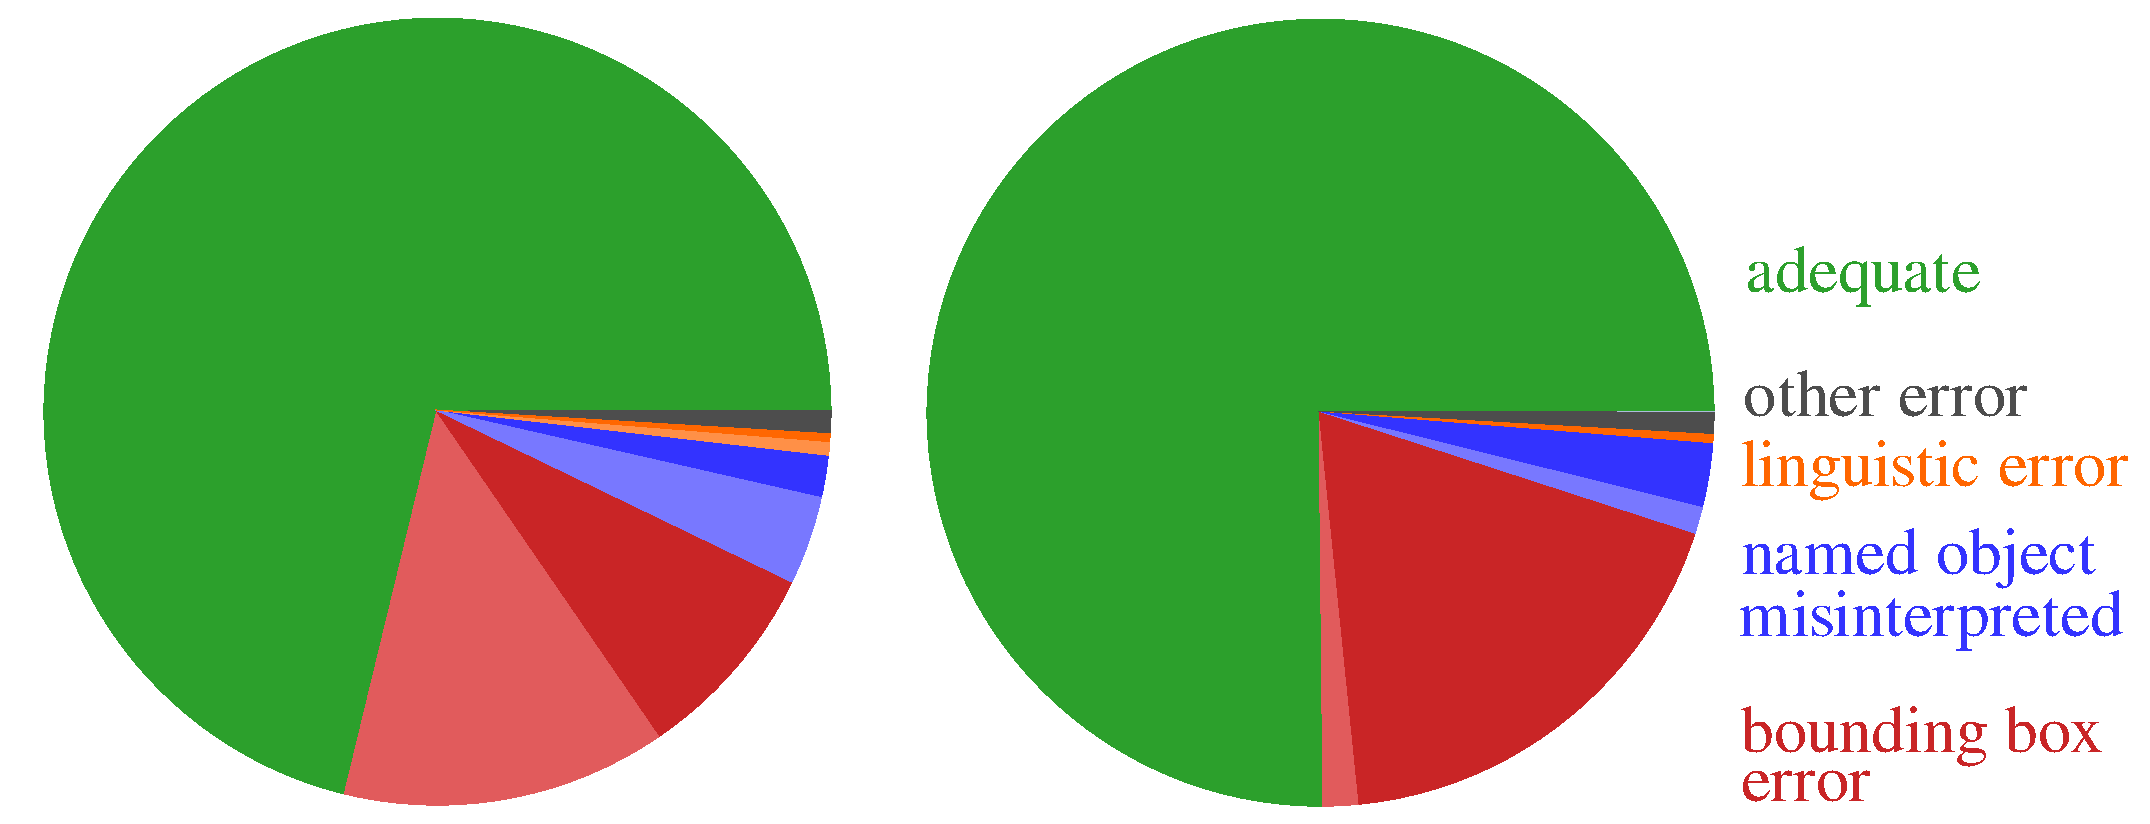
\includegraphics[width=\columnwidth]{images/verification_piechart_double.pdf}\\
% 	\hspace*{\fill}a.\hspace*{\fill}\hspace*{\fill}b.\hspace*{\fill}\hspace*{\fill}
% 	\caption{Verification results: a. counting individual annotations; b. counting image-name pairs with their aggregated scores. Lighter shade within a hue indicates slight/possible error of that type; darker shade severe error.}
% 	\label{fig:verification-piechart}
% \end{figure}


%%% Local Variables:
%%% mode: plain-tex
%%% TeX-master: "acl2020_main"
%%% End:
